\documentclass{beamer}

\usepackage[utf8]{inputenc} % Language and font encoding
\usepackage[icelandic]{babel}
\usepackage[T1]{fontenc}


\usepackage{tikz}
\usepackage[listings,theorems]{tcolorbox}
\usepackage{booktabs}
\usepackage{minted} %Minted and configuration
\usemintedstyle{default}

\renewcommand{\theFancyVerbLine}{\sffamily \arabic{FancyVerbLine}}
%%%%%%%%%%%
% More math
%%%%%%%%%%%
\newcommand{\Mod}[1]{\ \text{mod}\ #1}

%%%%%%%%%%%%%%%%%%%%%%
% Beamer configuration
%%%%%%%%%%%%%%%%%%%%%%
\setbeamertemplate{navigation symbols}{}
\usecolortheme{dove}
\setbeamercolor{frametitle}{fg=white}

\usebackgroundtemplate%
{%
\vbox to \paperheight{

\includegraphics[width=\paperwidth]{Pics/hi-slide-head-2016}

\vfill
\hspace{0.5cm}
\includegraphics[width=0.3\paperwidth]{Pics/hi-von-logo}
\vspace{0.4cm}
    }%
}

\AtBeginSection[]
{
  \begin{frame}<beamer>
    \frametitle{Yfirlit}
    \tableofcontents[currentsection]
  \end{frame}
}

\setbeamerfont{frametitle}{size=\normalsize}
\addtobeamertemplate{frametitle}{}{\vspace*{0.5cm}}

%%%%%%%%%%%%%%%%%%%%%%%%%
% tcolorbox configuration
%%%%%%%%%%%%%%%%%%%%%%%%%

% Setup from: http://tex.stackexchange.com/a/43329/21638
\tcbset{%
    noparskip,
    colback=gray!10, %background color of the box
    colframe=gray!40, %color of frame and title background
    coltext=black, %color of body text
    coltitle=black, %color of title text 
    fonttitle=\bfseries,
    alerted/.style={coltitle=red, colframe=gray!40},
    example/.style={coltitle=black, colframe=green!20, colback=green!5},
}


%%%%%%%%%%%%%%%%%%%%%%%
% Further configuration
%%%%%%%%%%%%%%%%%%%%%%%
\hypersetup{colorlinks=true,pdfauthor={Eirikur Ernir Thorsteinsson},linkcolor=blue,urlcolor=blue}
\graphicspath{{./Pics/}}

\author{Eiríkur Ernir Þorsteinsson}
\institute{Háskóli Íslands}
\date{Haust 2016}

\title{Stærðfræðimynstur í tölvunarfræði}
\subtitle{Vika 1, fyrri fyrirlestur}

\begin{document}

\begin{frame}
\titlepage
\end{frame}

\section{Um námskeiðið}

\begin{frame}{Tímar}
\begin{itemize}
 \item Fyrirlestrar
 \begin{itemize}
  \item Þriðjudögum klukkan 15:00 í HT-105, föstudögum klukkan 8:20 í HT-102
  \item Fyrirlestrar fara hratt yfir efni bókarinnar
 \end{itemize}
 \item Dæmatímar
 \begin{itemize}
  \item Hefjast í \emph{næstu viku}
  \item Sjö hópar, miðvikudögum til föstudaga
  \item Ykkur verður úthlutað hópum fljótlega\textsuperscript{\textregistered}
 \end{itemize}
\end{itemize} 
\end{frame}

\begin{frame}{Námsmat}
Einkunn ákvarðast af prófseinkunn og vetrareinkunn
\begin{columns}
\column{0.5\textwidth}
\begin{itemize}
 \item Prófseinkunn skiptist í lokaprófseinkunn og miðmisserisprófseinkunn
 \item Lokaprófseinkunn er 50\% og miðmisserisprófseinkunn 20\%
 \item Undantekning: lokaprófseinkunn gildir 70\% sé hún hærri en miðmisserisprófseinkunn, sem gildir þá 0\%
\end{itemize}
\column{0.5\textwidth}
\begin{itemize}
 \item Vetrareinkunn skiptist í skilaverkefnaeinkunn og tímaverkefnaeinkunn
 \item Skilaverkefnaeinkunn gildir 20\% af heildareinkunn
 \item Tímaverkefnaeinkunn gildir 10\% af heildareinkunn
\end{itemize}
\end{columns}
\end{frame}

\begin{frame}{Álag}
Námskeiðið er $8 ECTS$ einingar. 60 ECTS einingar eru skilgreindar sem 1500-1800 klst. af vinnu.
\[
\text{60 ECTS = 1650 klst.} \Longleftrightarrow \text{8 ECTS = 220 klst.}
\]
Misserið er 14 vikur, svo gera má ráð fyrir 15-16 klst. af vinnu í viku. Þar af eru 4 klst. í fyrirlestrum og dæmatímum.
\end{frame}


\begin{frame}{Kennari}
\begin{columns}
\column{0.5\textwidth}
\begin{itemize}
 \item Nafn: Eiríkur Ernir Þorsteinsson
 \item Aðsetur: Tæknigarði, 2. hæð, herbergi 214
 \item Tölvupóstfang: \href{mailto:eth31@hi.is}{eth31@hi.is}
 \begin{itemize}
  \item Sjá einnig: \hyperlink{frame:piazza}{Piazza}
 \end{itemize}
 \item Sími: 6994392
\end{itemize}
\column{0.5\textwidth}
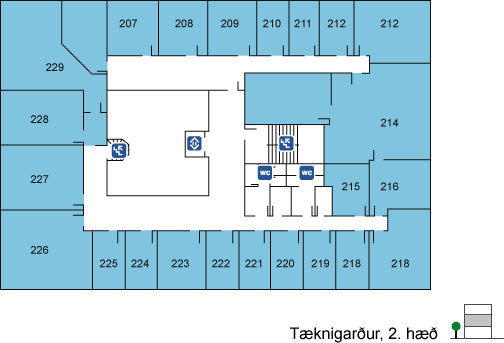
\includegraphics[width=\linewidth]{taeknigardur}
\end{columns}
\end{frame}

\section{Námefni og tól}

\begin{frame}{Kennslubók námskeiðsins}
\begin{columns}
\column{0.5\textwidth}
\begin{itemize}
 \item Nokkrar leiðir til að nálgast kennslubók og tilheyrandi efni
 \begin{itemize}
  \item Kaupa bók úr pappír (fæst í Bóksölu stúdenta), vefbók og æfingaaðgangur fylgir með
  \item Kaupa vefbók og æfingaaðgang á vefsíðu
  \item Kaupa æfingaaðgang eingöngu
 \end{itemize}
\end{itemize}
\column{0.5\textwidth}
\begin{center}
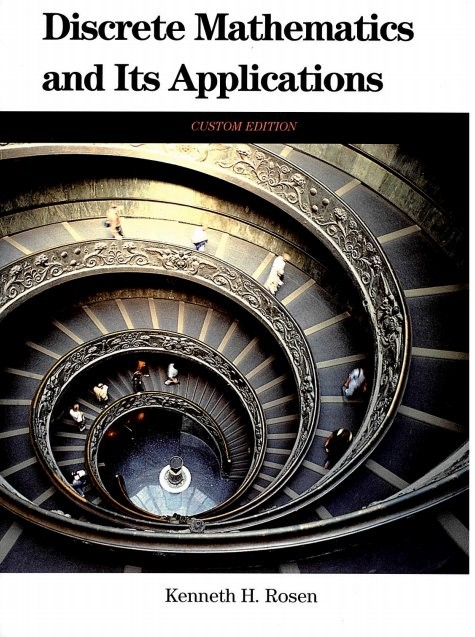
\includegraphics[width=0.7\linewidth]{Pics/rosen}
\end{center}
\end{columns}
\end{frame}

\begin{frame}{Connect}
\begin{itemize}
 \item Kennslusíða bókarinnar, \href{http://connect.mheducation.com/class/tol104g16}{McGraw-Hill Connect} verður notuð í dæmatímum og fyrirlestrum
 \begin{itemize}
  \item Æfingaverkefni sem fara yfir sig sjálf 
  \item Athugið að kaupa þarf aðgang!
 \end{itemize}
\end{itemize}
\end{frame}

\begin{frame}{Gradescope}
\begin{itemize}
 \item Verkefnaskil fara fram í vefkerfinu \href{https://gradescope.com/}{Gradescope}
 \item Kerfið tekur við \texttt{.pdf} skrám
 \item Fyrstu skilin munu koma í næstu viku
\end{itemize}
\end{frame}

\begin{frame}{Fyrirspurnir og umræður}
\label{frame:piazza}
\begin{itemize}
 \item Spjallkerfið \href{piazza.com/hi.is/fall2016/tl105g}{Piazza} verður notað í þessu námskeiði
 \item Kerfið mun vera besta leiðin til að fá svör frá samnemendum, dæmatímakennurum og undirrituðum
 \item Setjið allar fyrirspurnir um námskeiðið þangað!
 \begin{itemize}
  \item Kemur í stað tölvupósts
 \end{itemize}
\end{itemize}
\end{frame}

\subsection{Heilræði}

\begin{frame}{Heilræði}
\pause
\begin{itemize}
 \item Takið þátt í tímum\pause
 \item Gerið dæmin \pause
 \item Nýtið aðstoð 
 \begin{itemize}
  \item Piazza!
  \item Nemendafélög og lengra komnir nemar
  \item Námsráðgjöf HÍ \pause
 \end{itemize}
 \item Sofið og slakið á
\end{itemize}
\end{frame}

\section{Yrðingar}

\begin{frame}{Yrðingar}
\begin{tcolorbox}[title=Yrðing]
Yrðing (e. \emph{proposition}) er fullyrðing sem er áreiðanlega sönn eða ósönn.
\end{tcolorbox}
\begin{columns}
\column{0.6\textwidth}
\begin{itemize}
 \item Dæmi um yrðingar:
 \begin{itemize}
  \item Við erum stödd í stofu HT-105
  \item $2 + 2 = 4$
  \item $1 + 2 = 5$
 \end{itemize}
\end{itemize}
\column{0.4\textwidth}
\begin{itemize}
 \item Ekki dæmi um yrðingar:
 \begin{itemize}
  \item Lokaðu hurðinni!
  \item Hvað er klukkan?
 \end{itemize}
\end{itemize}
\end{columns}
\end{frame}

\begin{frame}{Yrðingar}
\begin{tcolorbox}[title=Yrðing]
Yrðing (e. \emph{proposition}) er fullyrðing sem er áreiðanlega sönn eða ósönn.
\end{tcolorbox}
\begin{itemize}
 \item Ekki yrðingar (órætt)
 \begin{itemize}
  \item $x + 1 = 2$
  \item $x + y = z$
 \end{itemize} \pause
 \item Mætti breyta þessu í yrðingar?\pause
 \begin{itemize}
  \item Já, með því að gefa breytunum $x$, $y$ og $z$ gildi
 \end{itemize}
\end{itemize}
\end{frame}

\begin{frame}{Yrðingabreytur}
\begin{itemize}
 \item Hægt er að nota yrðingabreytur (e. \emph{propositional variables}) til að tákna yrðingar
 \begin{itemize}
  \item Alveg hliðstætt því að nota breytur til að geyma gildi á tölum
 \end{itemize}
 \item Oftast eru stafirnir $p, q, r$ og $s$ notaðir til að tákna yrðingabreytur
 \item Yrðinguna sem er alltaf sönn má tákna með $T$ eða 1, yrðinguna sem er alltaf ósönn má tákna með $F$ eða 0
 \item Hægt er að nota yrðingabreytur til að framkvæma yrðingareikninga (e. \emph{propositional calculus})
\end{itemize}
\end{frame}

\begin{frame}{Samsettar yrðingar}
\begin{itemize}
 \item Samsett yrðing (e. \emph{compound proposition}) er búin til með því að nota smærri yrðingar og rökvirkja (e. \emph{logic operators})
 \item Rökvirkjarnir og táknin sem notaðir eru fyrir þau:
 \begin{itemize}
  \item Neitun, $\lnot$ (e. \emph{negation})
  \item Og-un, $\land$ (e. \emph{conjunction})
  \item Eð-un, $\lor$ (e. \emph{disjunction})
  \item Afleiðing, $\to$ (e. \emph{implication})
  \item Jafngildi $\leftrightarrow$ (e. \emph{biconditional})
 \end{itemize}
\end{itemize}
\end{frame}

\begin{frame}{Neitun}
Dæmi um neitun: Ef $p$ stendur fyrir ``við erum stödd í stofu HT-105'', þá stendur $\lnot p$ fyrir ``það er ekki svo að við séum stödd í stofu HT-105'' (sem umorða má í ``við erum ekki stödd í stofu HT-105'').

\vspace*{0.5cm}
Sanntafla (e. \emph{truth table}) neitunar:

\begin{center}
\begin{tabular}{ll}
\toprule
$p$&$\lnot p$\\
\midrule
0&1\\
1&0\\
\bottomrule
\end{tabular}
\end{center}
\end{frame}

\begin{frame}{Og-un}
\begin{columns}
\column{0.6\textwidth}
Samsett yrðing búin til með og-un er sönn þegar báðar yrðingarnar sem að henni koma eru sannar.

\vspace*{0.5cm}
Hvert er sanngildi samsettu yrðingarinnar ``við erum stödd í stofu HT-105 og við erum að læra Stærðfræðimynstur''? En yrðingarinnar ``við erum stödd í stofu HT-105 og við erum að læra Tölvutækni og samfélagið''?
\column{0.4\textwidth}
Sanntafla og-unar:
\begin{center}
\begin{tabular}{ccc}
\toprule
$p$&$q$&$p \land q$ \\
\midrule
1&1&1\\
1&0&0\\
0&1&0\\
0&0&0\\
\bottomrule
\end{tabular}
\end{center}
\end{columns}
\end{frame}

\begin{frame}{eð-un}
\begin{columns}
\column{0.6\textwidth}
Samsett yrðing búin til með eð-un er sönn þegar a.m.k. önnur yrðingin sem að henni kemur er sönn.

\vspace*{0.5cm}
Hvert er sanngildi samsettu yrðingarinnar ``við erum stödd í stofu HT-105 eða við erum að læra Tölvutækni og samfélagið''?
\column{0.4\textwidth}
Sanntafla eð-unar:
\begin{center}
\begin{tabular}{ccc}
\toprule
$p$&$q$&$p \lor q$ \\
\midrule
1&1&1\\
1&0&1\\
0&1&1\\
0&0&0\\
\bottomrule
\end{tabular}
\end{center}
\end{columns}
\end{frame}


\end{document}
